
\newpage

\section{Usage}

The application is available for using online,
and can be accessed online at \url{http://math.random.fi/scheduler/},
and the source code is available online at \url{https://github.com/dtinth/scheduler}.

\subsection{The Main Application Window}

After entering the web application,
you will see a blank schedule, as seen in \autoref{fig:usage-intro}:

\begin{figure}[h]
  \centering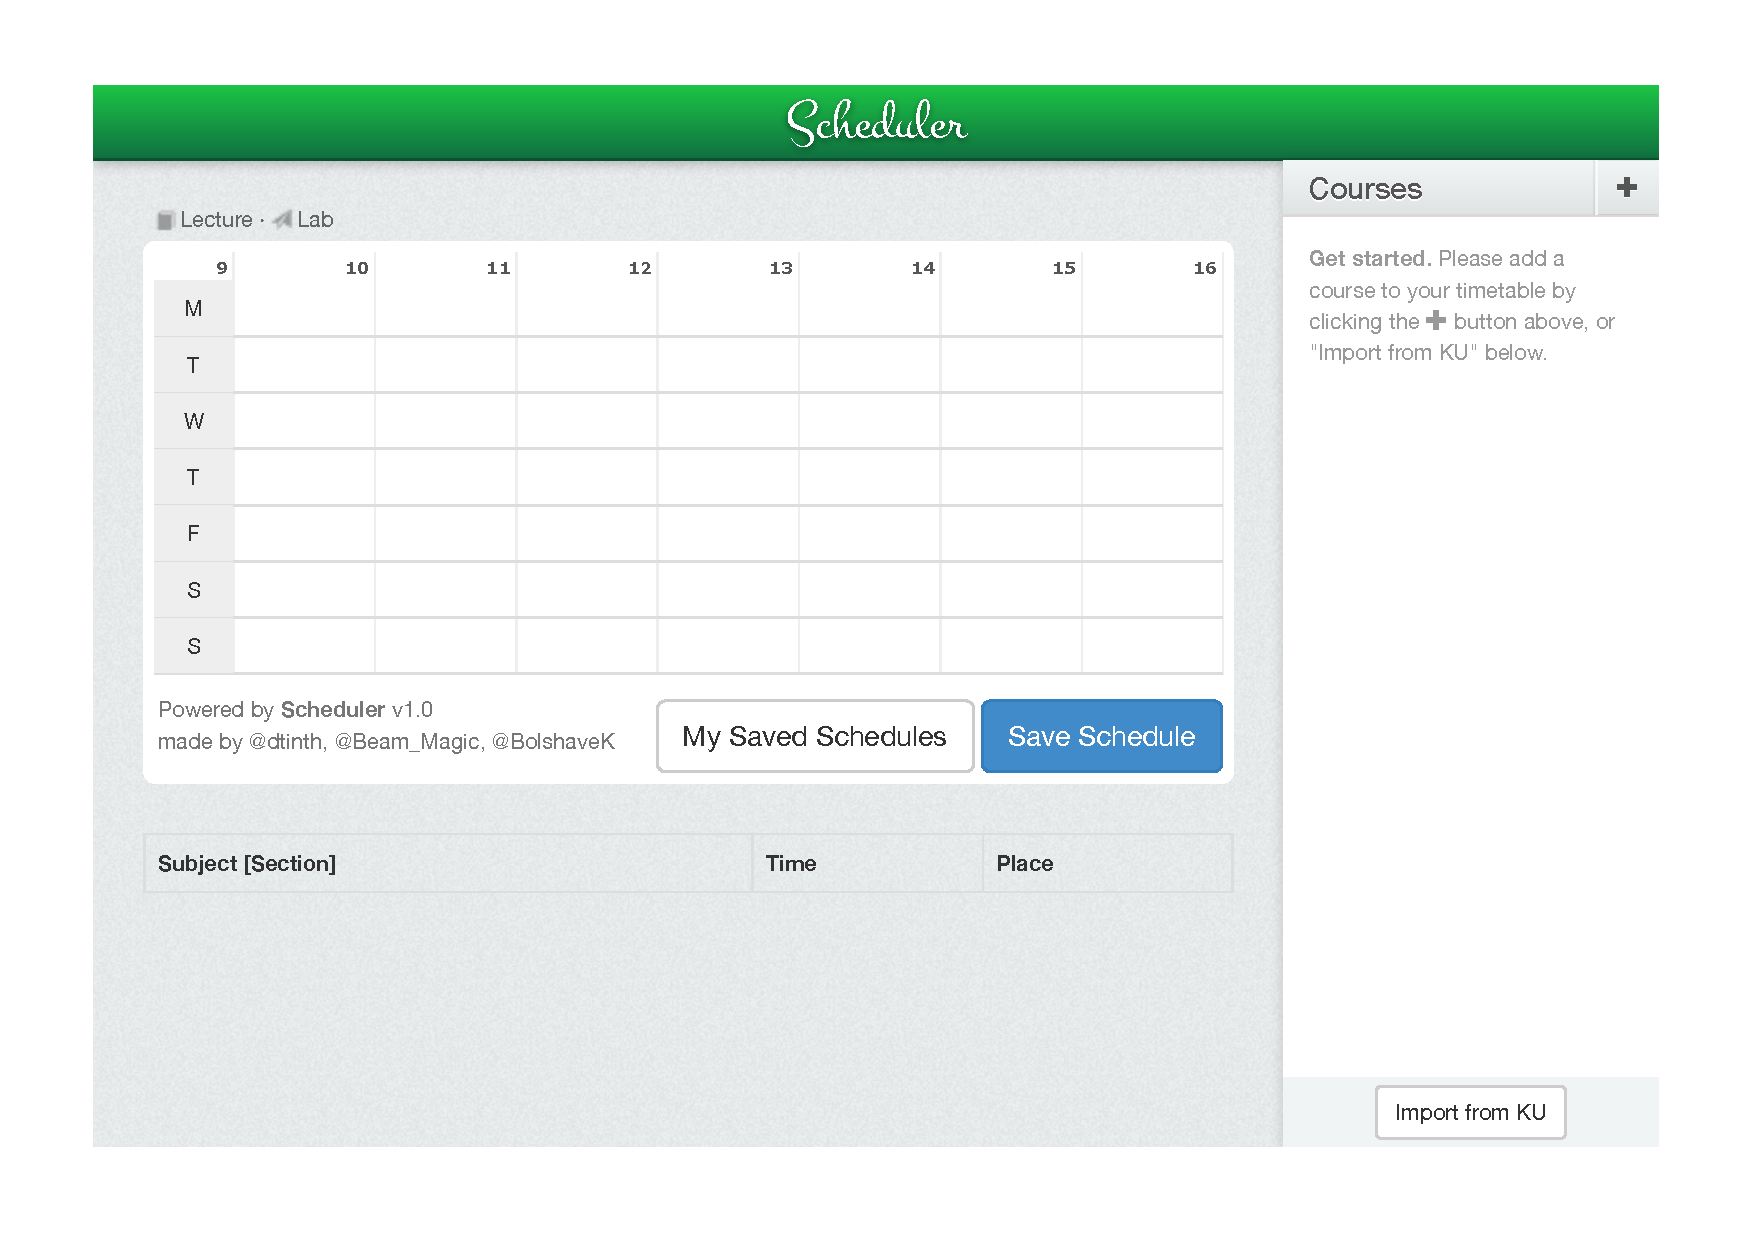
\includegraphics[width=0.8\textwidth]{../../images/usage-intro.pdf}
  \caption{A blank schedule, which is what you see when you first enter the application}
  \label{fig:usage-intro}
\end{figure}

\begin{itemize}
  \item
    Clicking the small plus-sign button at the top-right of the screen
    creates a new course and opens an editor window for you to edit it.
  \item
    Clicking the \emph{Import from KU} button will open a dialog box
    that lets you import schedule data from Kasetsart University's registration system.
    (See \autoref{subsec:import})
  \item
    The right side of the screen shows the available courses.
    You can add a course to your personal schedule by clicking on the section number.
  \item
    The main part of the screen shows your personal schedule.
\end{itemize}


\subsection{The Import Window}
\label{subsec:import}

After clicking the \emph{Import from KU} button,
a new window for importing will appear, as seen in \autoref{fig:usage-import}.

\begin{itemize}
  \item
    Type the course name or the course code in the search field.
  \item
    Select the semester to import the schedule of that course.
  \item
    Clicking the course code in the result table imports it into your schedule.
\end{itemize}

\subsection{Course Info Editor}
\label{subsec:course}

When creating a new course
(by clicking the plus button at the top of then main window)
or editing a course
(by clicking the course name),
a course editor window will appear, as seen in \autoref{fig:usage-course}.
Any changes are saved and reflected in your timetable immediately.

\begin{itemize}
  \item
    You can change the course ID (course code),
    course name,
    and the number of lecture and lab credits for this course
    by editing the fields at the top.
  \item
    Clicking the green \emph{Add Section} button in the toolbar at the bottom
    adds another section to this course.
  \item
    Clicking the $\times$ at the right of a section header
    removes that section from this course.
  \item
    Clicking the green plus sign in the timetable
    adds a new period to the schedule for that section.
  \item
    Clicking the red $\times$ button in the timetable
    removes that period from that section.
  \item
    Clicking the red \emph{Remove} button in the toolbar at the bottom
    removes the whole course from your timetable,
    and closes the editor.
  \item
    Clicking the blue \emph{Close} button in the toolbar at the bottom
    closes the editor.
\end{itemize}

After importing, adding, and editing courses, sections and their periods,
you will see them on the right-hand side of the screen (see \autoref{fig:usage-finish}).

\begin{itemize}
  \item
    Click on the section number at the right to put it on your personal timetable.
  \item
    Click on the course name at the right to edit that course information.
  \item
    Click on the course name in your personal timetable
    to change its display name.
    This is useful when the course name is very long.
\end{itemize}

\begin{figure}[h]
  \centering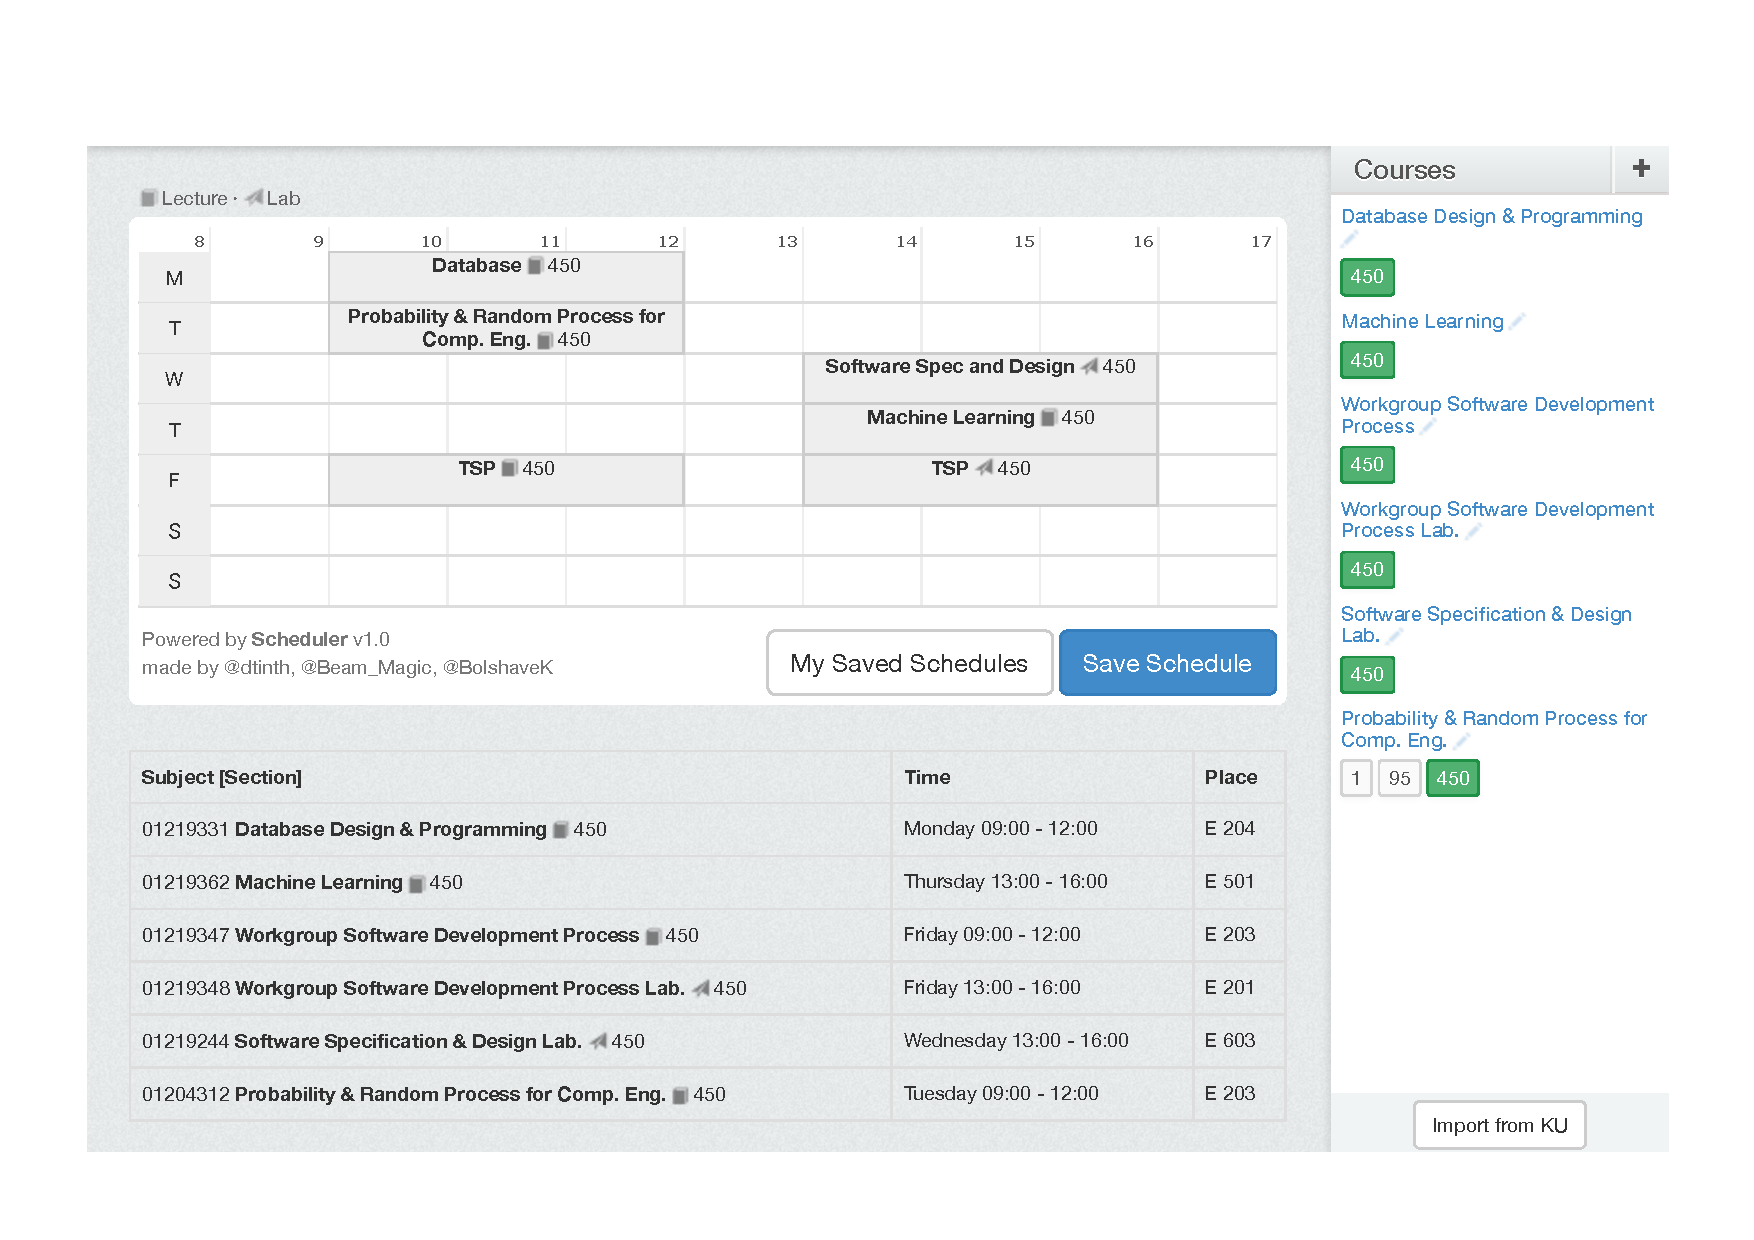
\includegraphics[width=0.75\textwidth]{../../images/usage-finish.pdf}
  \caption{A finished schedule.}
  \label{fig:usage-finish}
\end{figure}

\begin{figure}[p]
  \centering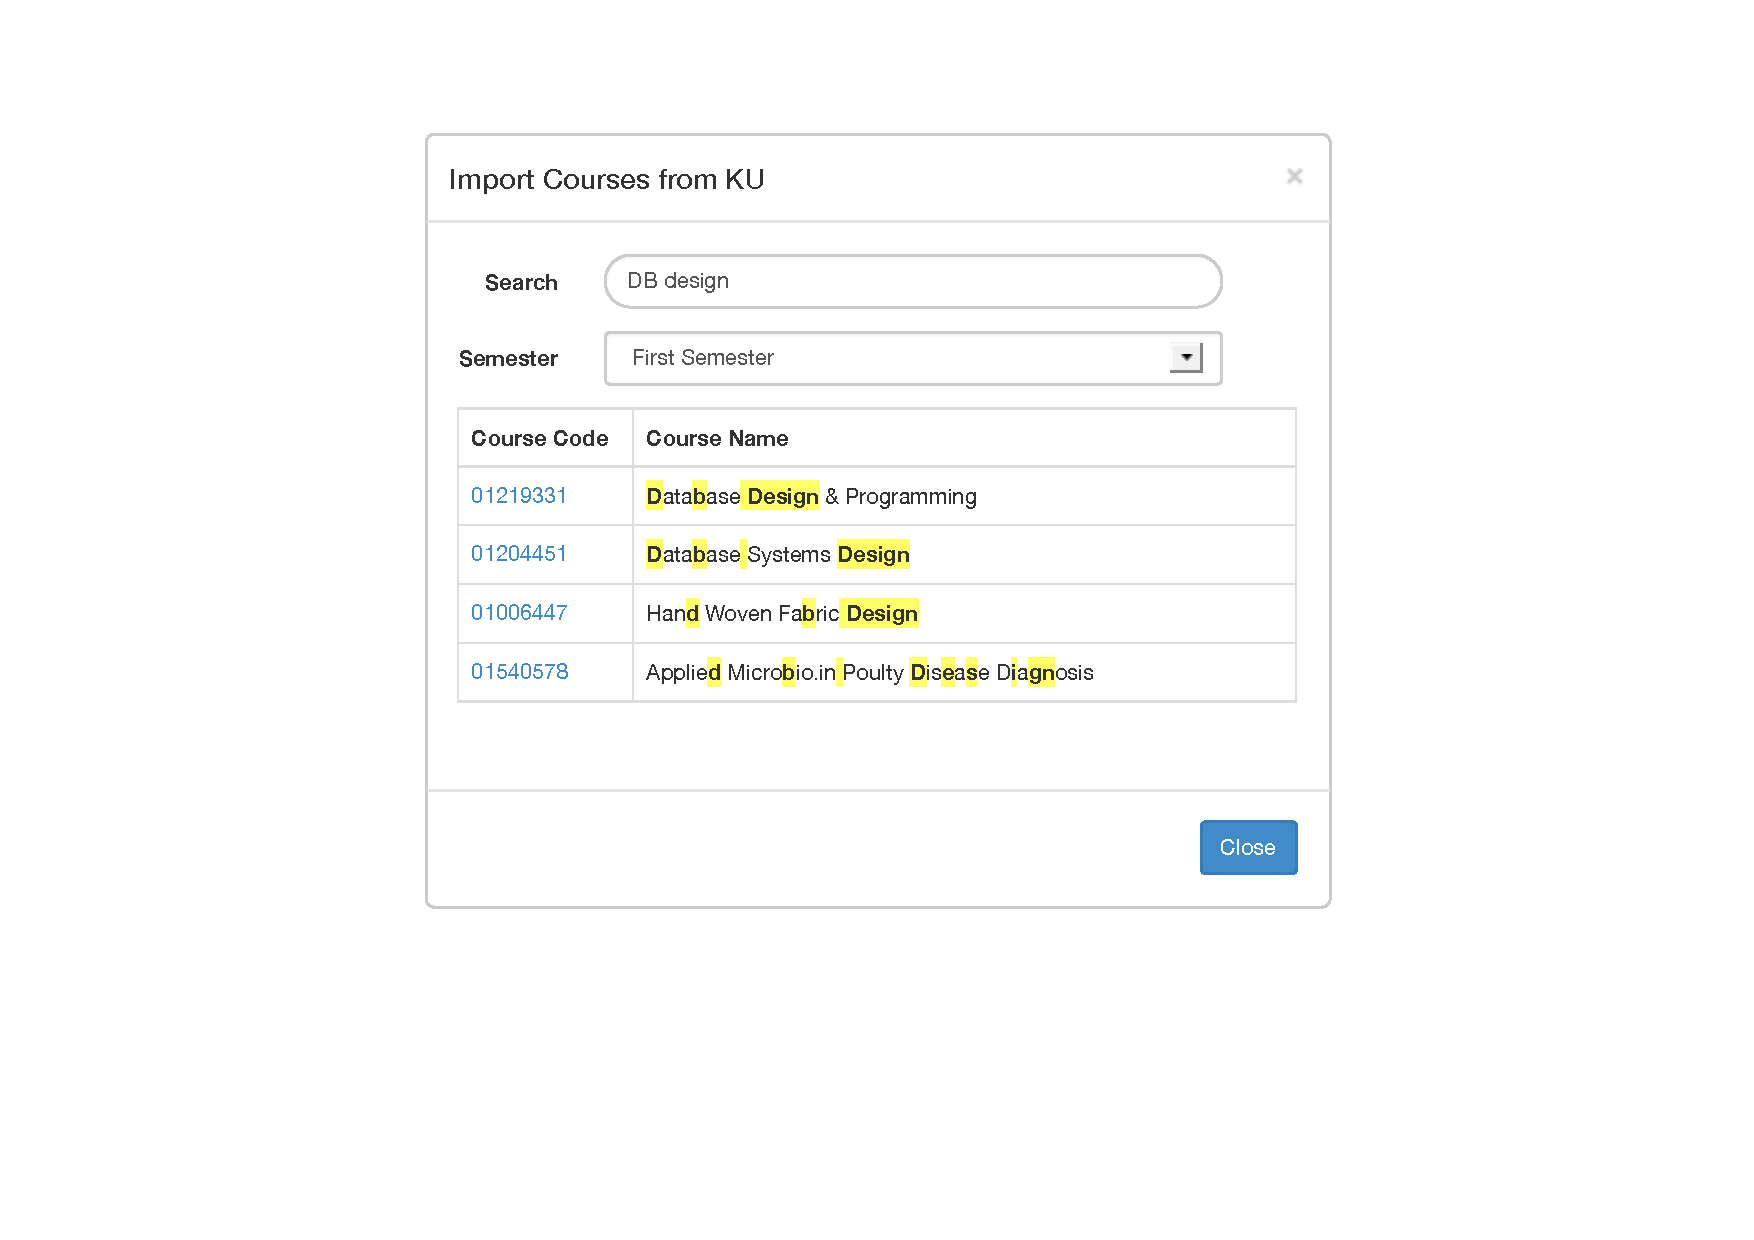
\includegraphics[width=0.6\textwidth]{../../images/usage-import.pdf}
  \caption{The import window,
    which lets you type in the course name or course ID
    to search for the course you desire to import.}
  \label{fig:usage-import}
\end{figure}

\begin{figure}[p]
  \centering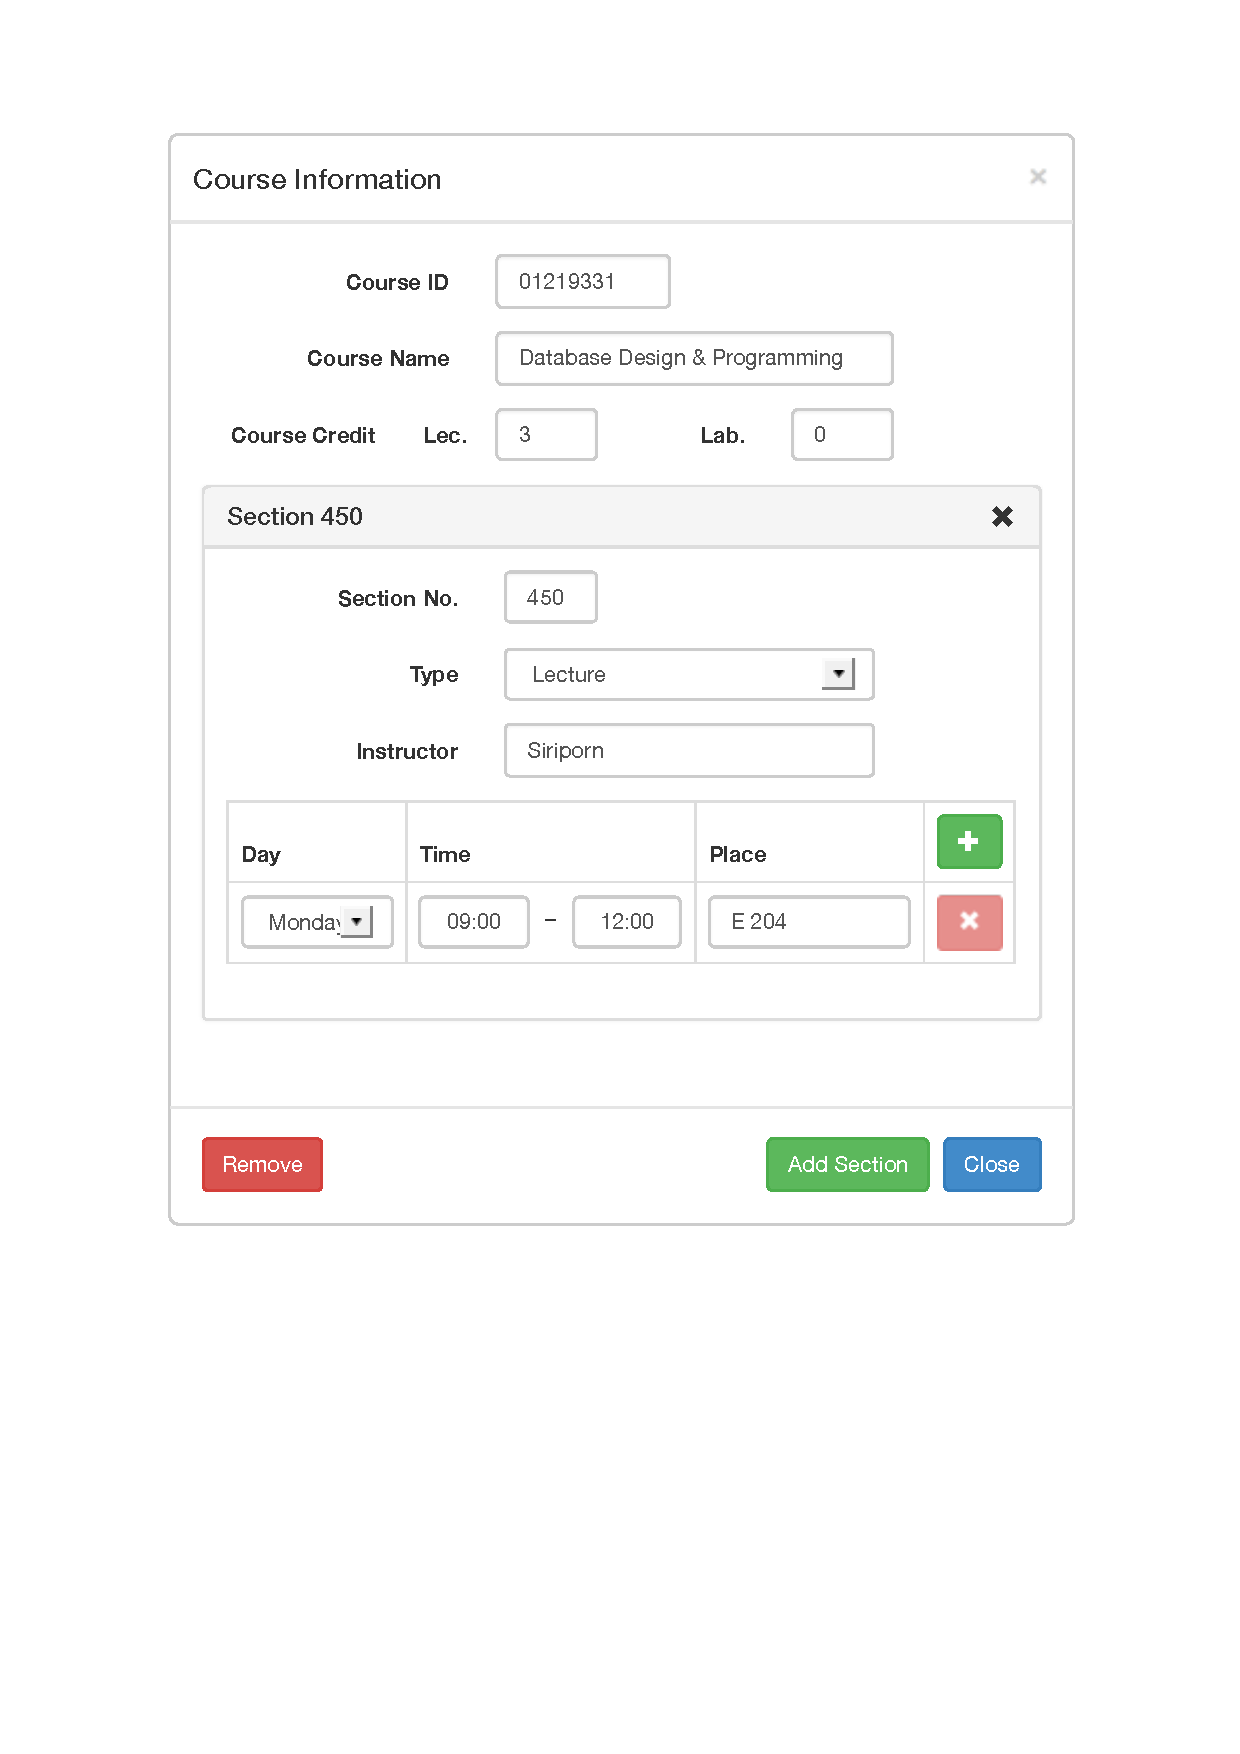
\includegraphics[width=0.6\textwidth]{../../images/usage-course.pdf}
  \caption{The course editor,
    which lets you edit the information for a single course.}
  \label{fig:usage-course}
\end{figure}


\FloatBarrier
\subsection{Saving your Schedule}
\label{subsec:save}

Please note that nothing is saved to the database
until you click the \emph{Save Schedule} button
and filled all the required information in.

When clicking the Save button, you will see a Save dialog,
as can be seen in \autoref{fig:usage-save}.

\begin{figure}[h]
  \centering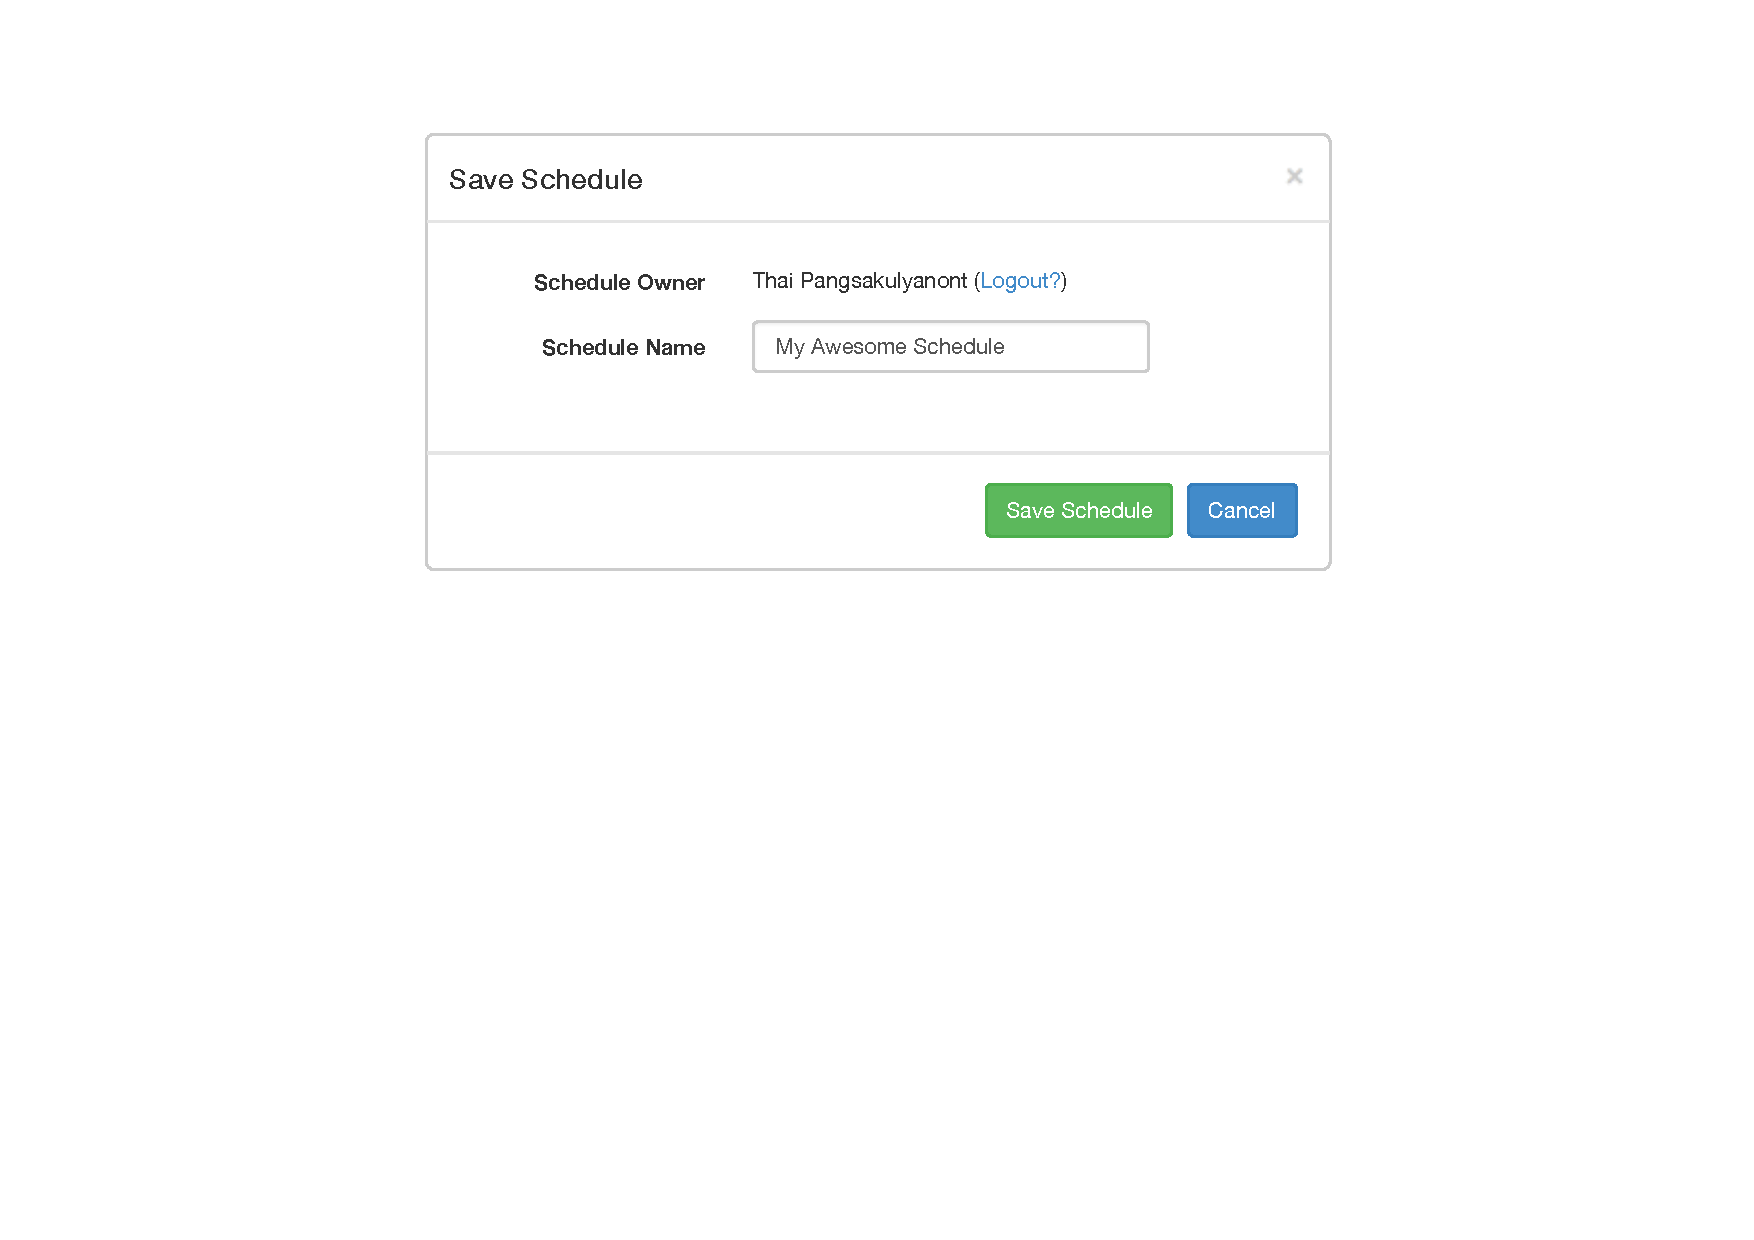
\includegraphics[width=0.7\textwidth]{../../images/usage-save.pdf}
  \caption{The save dialog.}
  \label{fig:usage-save}
\end{figure}

\begin{figure}[b!]
  \centering\fbox{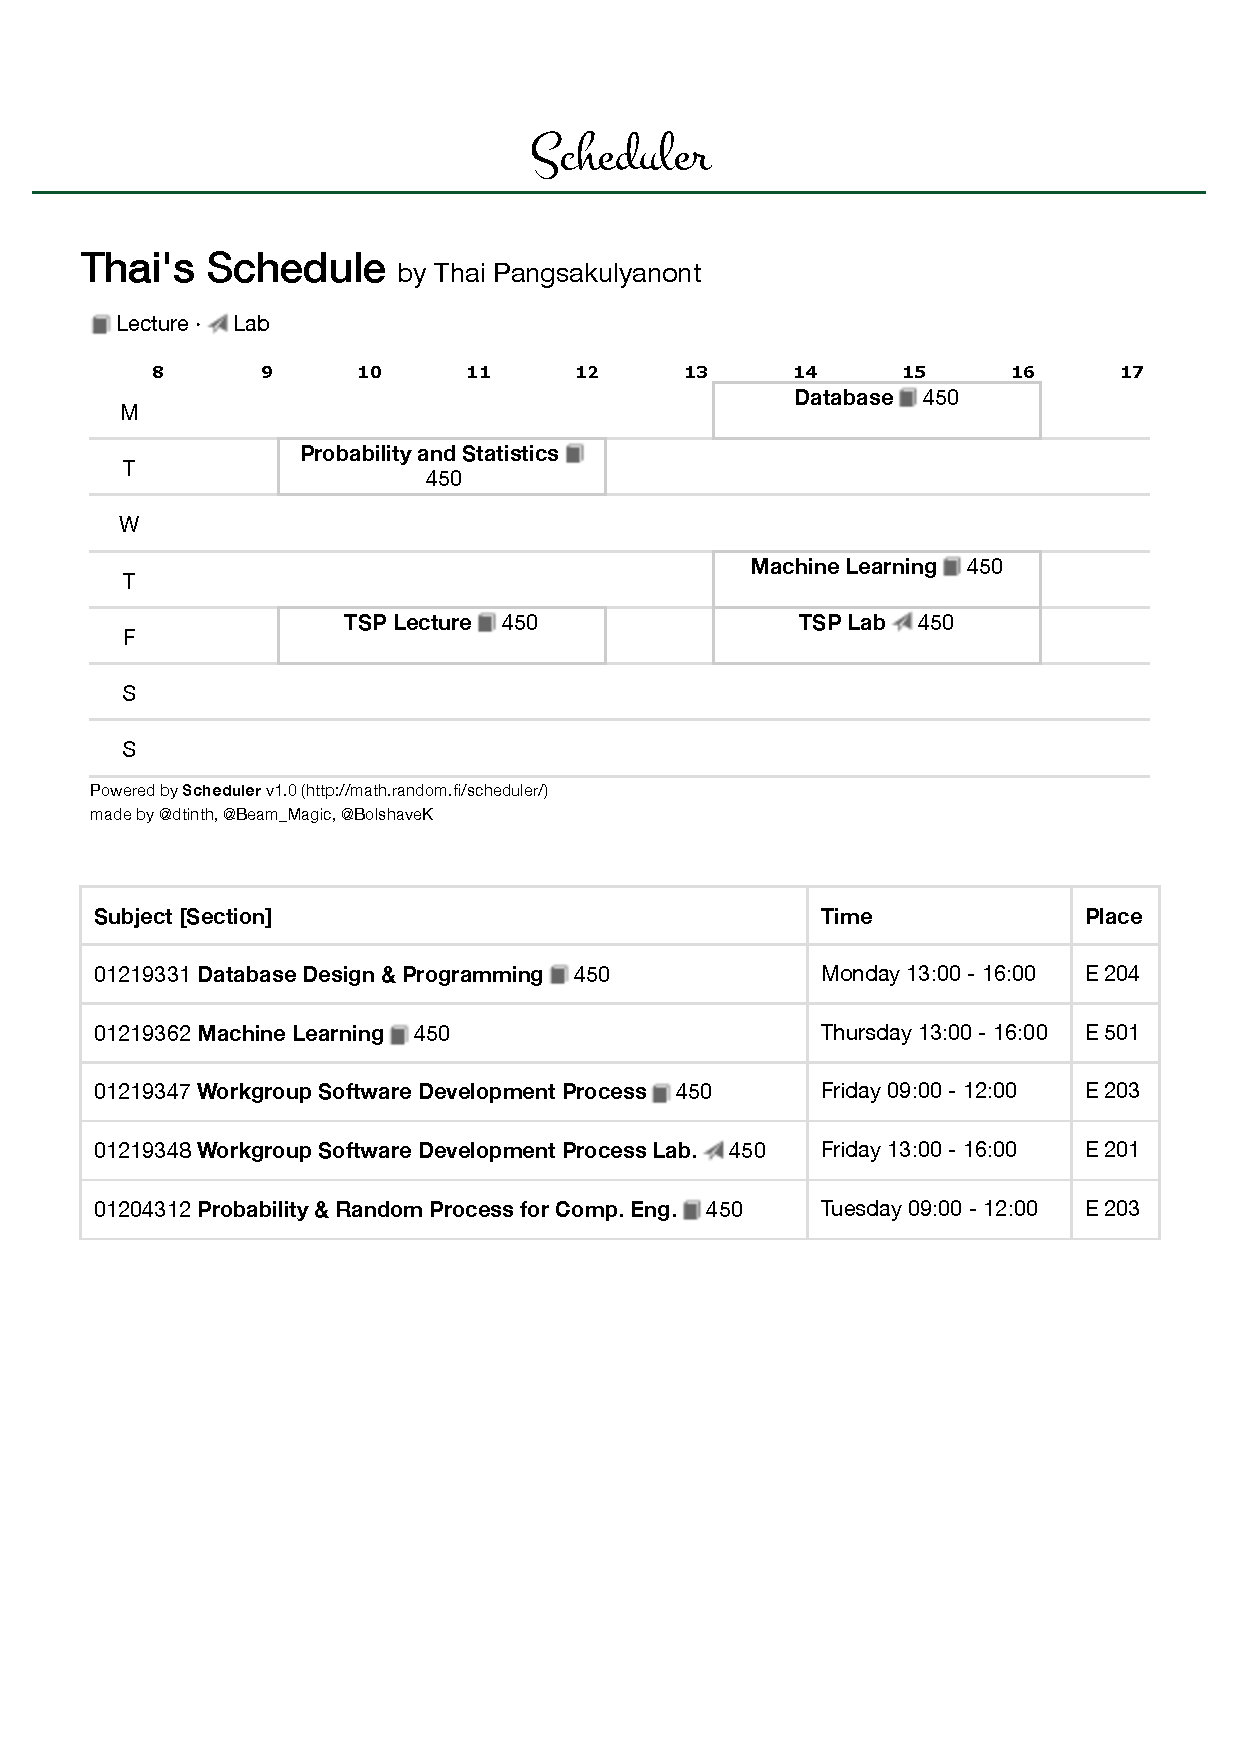
\includegraphics[width=0.7\textwidth]{../../images/usage-done.pdf}}
  \caption{The print view of the schedule.}
  \label{fig:usage-done}
\end{figure}

\begin{itemize}
  \item
    Sign in with Facebook to make sure
    that your schedules are kept.
    Annonymous schedules may be deleted after a certain period of time.
  \item
    Type in the name of your schedule.
  \item
    Click the Save Schedule button to save your schedule to the database.
\end{itemize}


After saving,
Scheduler will redirect you to the view page
that lets you view your finished schedule.
You can share that link to other people,
or print the schedule by selecting Print from the file menu.
The example of a printed schedule can be seen in \autoref{fig:usage-done}.


\section{Installation}

This section contains the installation instructions
to install this software from the source code.

Please note again that this application is available online
at \url{http://math.random.fi/scheduler/}.


\subsection{Prerequisites}

To run the Scheduler web application in your development machine,
the following things are required:

\begin{itemize}
  \item A PHP-enabled web server, with PHP 5.4 or newer.
  \item A MySQL database.
  \item Installed Composer from \url{http://getcomposer.org/}.
  \item A Facebook developer account.
\end{itemize}



\subsection{Installation Instructions}

After obtaining the source code and all the required prerequisites,

\begin{enumerate}
  \item
    Create a database called \texttt{zp2925\_schedule} in your MySQL DBMS,
    and import the database schema from \texttt{schema.sql} into that database.
  \item
    Using your Terminal or Command Prompt,
    navigate to the \texttt{backend} folder.
    With composer installed, issue the following command:

    \begin{verbatim}    composer install\end{verbatim}

    This will create a folder called \texttt{vendor} inside your \texttt{backend} folder,
    then download and install all the required dependencies needed to run the software inside that folder.
  \item
    In the folder \texttt{backend/includes},
    duplicate the file named \texttt{database.local.example.php}
    and name it \texttt{database.local.php}.
    Inside that file,
    configure the username and password to access the database.
  \item
    These steps are required if you want to enable Facebook integration.
    For security and privacy concerns,
    you need to create your own application
    from Facebook's developers page (\url{https://developers.facebook.com/}).

    In the \emph{Select how your app integrates with Facebook},
    select \emph{Website with Facebook login},
    and enter into the \emph{Site URL} the URL where this application will be accessed (see \autoref{fig:facebook-dev})

    \begin{itemize}
      \item
        In the folder \texttt{backend/includes},
        duplicate the file named \texttt{facebook.local.example.php}
        and name it \texttt{facebook.local.php}.
        Inside that file,
        put the \emph{Application Secret} code into this file,
        following the given template.
      \item
        In the folder \texttt{backend/includes},
        modify the file \texttt{facebook.php}
        and change the \texttt{appId} to your application's App ID.

        The same goes for \texttt{facebook.js} inside the \texttt{js} folder.
    \end{itemize}
  \item
    Upload your files to the web server.

    You should now be able to run the application from your web server.
\end{enumerate}

\begin{figure}[t!]
  \centering\fbox{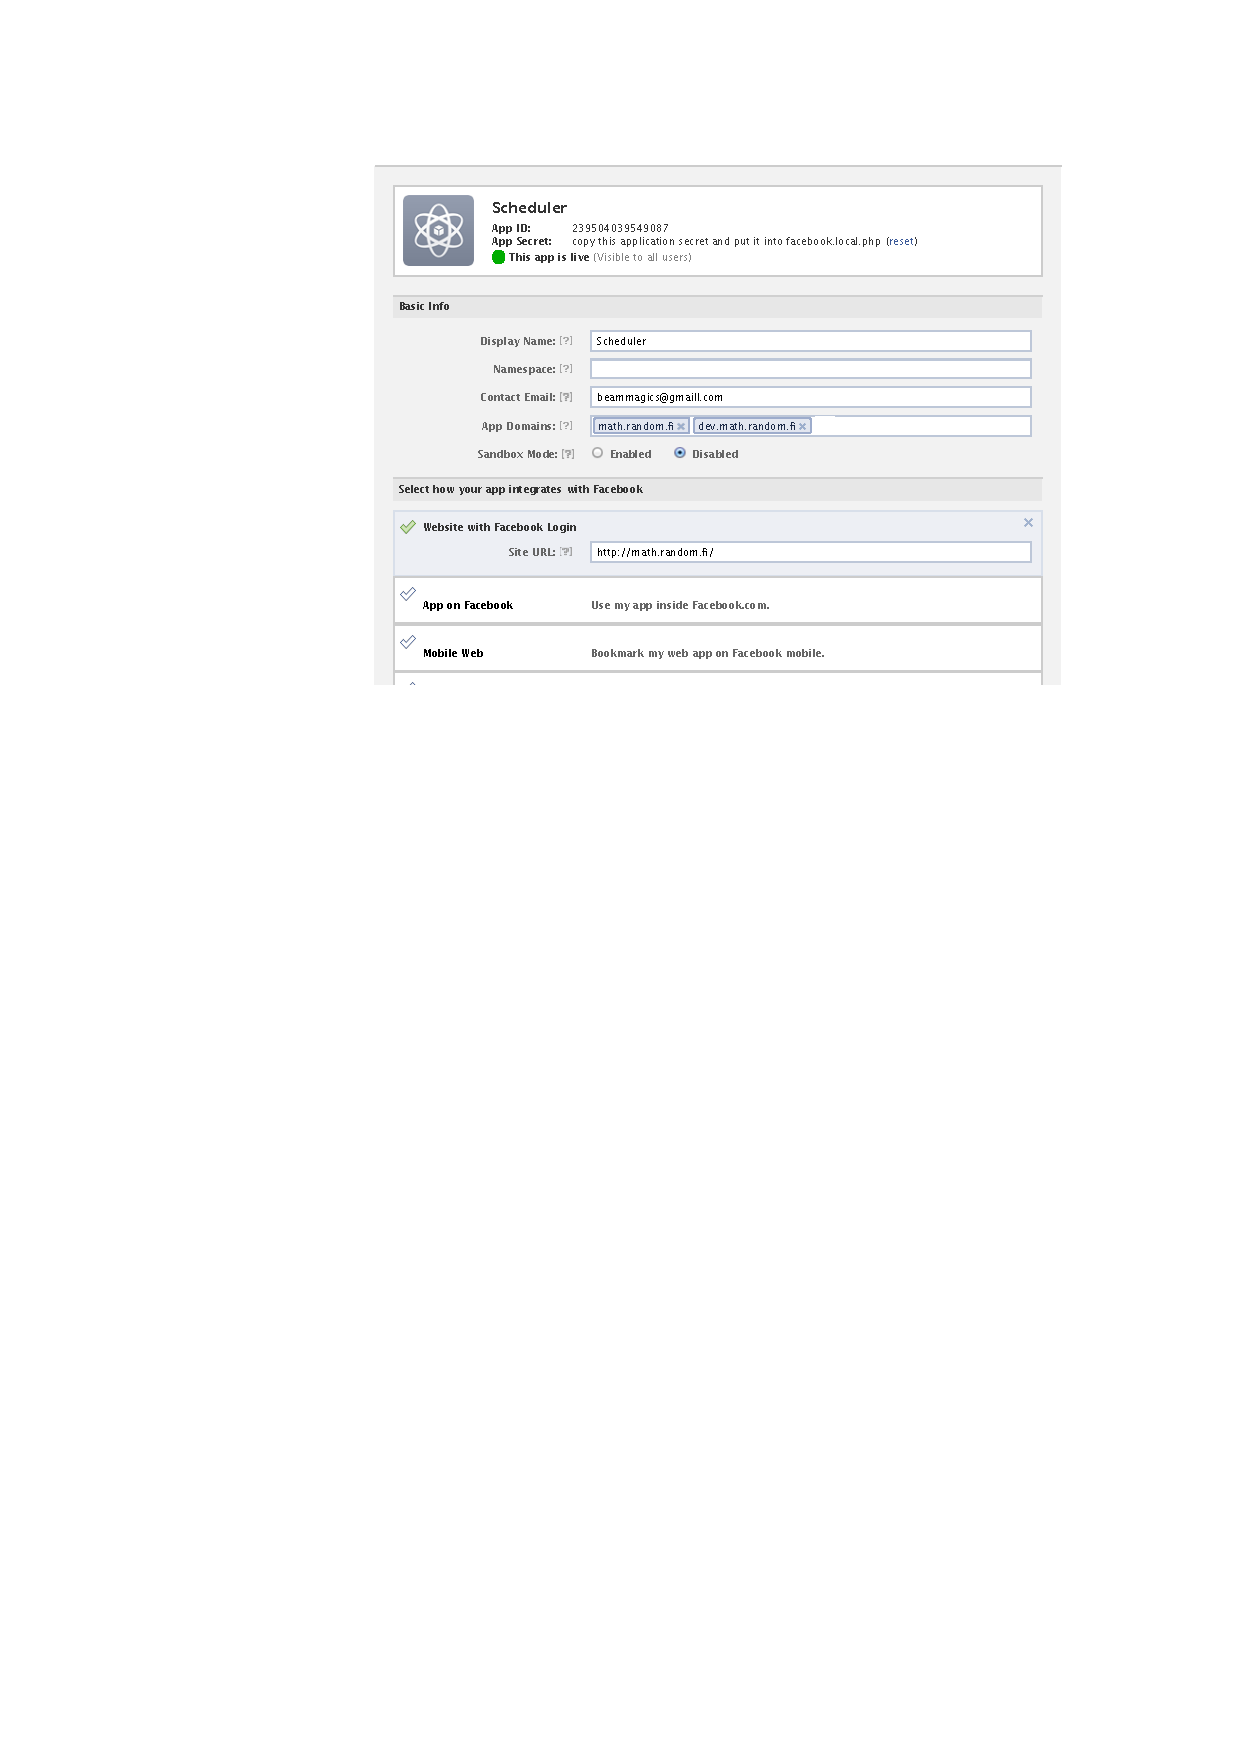
\includegraphics[width=0.9\textwidth]{../../images/installation-facebook.pdf}}
  \caption{An example Facebook application configuration.
    Note that the \emph{Website with Facebook login} is selected.}
  \label{fig:facebook-dev}
\end{figure}













